\documentclass[11pt]{article}

\usepackage{graphics} % or graphicx 
\usepackage{epstopdf}
\usepackage{multirow}
\usepackage{amsmath}
\usepackage{bbding}
\usepackage{pifont}
\usepackage{wasysym}
\usepackage{amssymb}
%%\usepackage[parfill]{parskip}



\setlength{\oddsidemargin}{0in}
\setlength{\textwidth}{6.5in}
\setlength{\topmargin}{-0.5in}
\setlength{\textheight}{8.75in}
\setlength{\parindent}{0pt}
\setlength{\parskip}{6pt}

\usepackage{fancyhdr}
\pagestyle{fancy}
\lhead{HW3}
\rhead{Reza Shisheie}

\usepackage{epsfig,graphicx}

\usepackage{amsmath}

\usepackage{clrscode3e}

\begin{document}

\thispagestyle{plain}

\begin{center}
{\Large \bf CIS 606 \hfil Homework 3 \hfil Fall 2019} \\
\end{center}

\vskip 1in 

\centerline{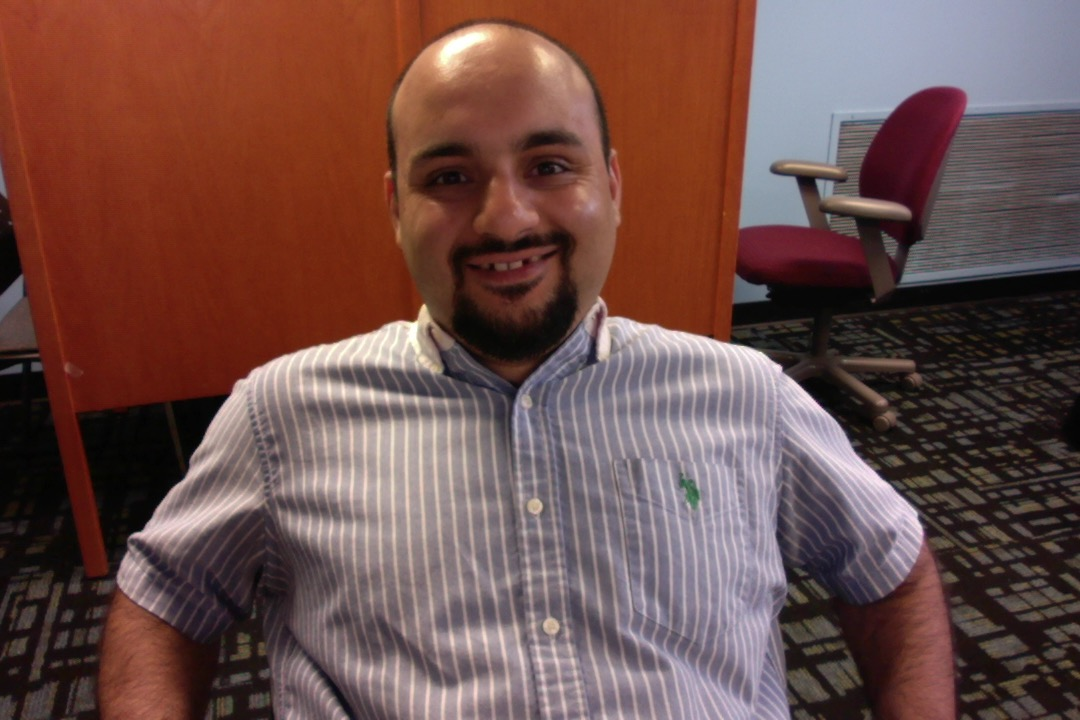
\includegraphics[width=3in]{photo.jpg}}

\vskip 0.5in 


\begin{center}
\begin{tabular}{ll}
{\bf Name:}     & {\bf Reza Shisheie } \\ \\
{\bf Login ID:} & {\bf reshishe }   
\end{tabular}
\end{center}

\newpage

\begin{enumerate}

\itemsep 0.35in

\item Exercise 4.2-6 (Textbook page 83): 
	
	Assuming 
	
	
	\hspace{10mm} \begin{math}
		A_{i}=
		\begin{bmatrix}
		  A_{i, 1\times 1}	&\cdots &A_{i, 1\times n}\\
		  \vdots			&\ddots &\vdots\\
		  A_{i, n\times 1}	&\cdots	&A_{i, n\times n}
		\end{bmatrix}_{n \times n}
		,
		B_{i}=
		\begin{bmatrix}
		  B_{i, 1\times 1}	&\cdots &B_{i, 1\times n}\\
		  \vdots			&\ddots &\vdots\\
		  B_{i, n\times 1}	&\cdots	&B_{i, n\times n}
		\end{bmatrix}_{n \times n}
		, 
		i \epsilon [1,...,k]
	\end{math}
	
	where, 
	
	\hspace{10mm} \begin{math}
		A=
		\begin{bmatrix}
		  A_{1}	\\
		  \vdots\\
		  A_{i}	
		\end{bmatrix}_{kn \times n}
		, 
		B=
		\begin{bmatrix}
		  B_{1}	&\cdots &B_{i}
		\end{bmatrix}_{n \times kn}
		, 
		i \epsilon [1,...,k]
	\end{math}
	
	
	\begin{itemize}
    	\item Forward Solution:

		Thus the product of $A \times B$ is a $kn \times kn$ matrix:
	
		\hspace{10mm} \begin{math}
			A \times B=
			\begin{bmatrix}
			  A_{1} \times B_{1} &\cdots & A_{1} \times B_{i}\\
			  \vdots			 &\ddots & \vdots\\
			  A_{i} \times B_{1} &\cdots & A_{i} \times B_{i}
			\end{bmatrix}_{kn \times kn}
		, 
			i \epsilon [1,...,k]
		\end{math}
	
		where time complexity of each $A_{i} \times B_{i}$ costs $\Theta(n^{\log_2{7}})$ according to Strassen's algorithm. Since there are $k^2$ matrix multiplications, time complexity of  $A \times B$ is:
	
		\hspace{10mm} $T(n)_{A \times B}=k^2.\Theta(n^{\log_2{7}})=\Theta(k^2.n^{\log_2{7}})$
	\end{itemize}
	
	\begin{itemize}
    	\item Reverse Solution:
		For the reverse multiplication, the product of $B \times A$ is a $n \times n$ matrix:
	
		\hspace{10mm} \begin{math}
			B \times A=
			\begin{bmatrix}
			  B_{1} \times A_{1}+ \cdots +B_{i} \times A_{i}
			\end{bmatrix}_{n \times n}
		\end{math}
		\begin{math}
			=
			\begin{bmatrix}
			  \sum_{i=1}^{k} {B_{i} \times A_{i}}
			\end{bmatrix}_{n \times n}
		\end{math}

		where time complexity of each $B_{i} \times A_{i}$ costs $\Theta(n^{\log_2{7}})$ according to Strassen's algorithm. Since there are $k$ matrix-multiplications in the summation, time complexity of  $B \times A$ is:
	
		\hspace{10mm} $T(n)_{B \times A}=k.\Theta(n^{\log_2{7}})=\Theta(k.n^{\log_2{7}})$


	\end{itemize}

	
	
	
	


\item Exercise 4.2-7 (Textbook page 83): 
	
	Assuming $A=a+bi$ and $B=c+di$, then $A.B$ is:
	
	\hspace{10mm} $A.B=(ac-bd)+(ad+bc).i$
    $ \overset{}{\implies}$
	$
	    \left\{\begin{array}{lr}
	    
        	\mathrm{Real} = (ac-bd)\\
        	\mathrm{Imag} = (ad+bc)
        \end{array}\right\}
    $ 


	Assuming $u$, $v$, and $w$ as follows: 
	
	\hspace{10mm} $ u = (a+b).(c+d)=ac+ad+bc+bd$;  // counts as 2 sum and 1 multiplication 
	
	\hspace{10mm} $ v = ac$;  // counts as 1 multiplication between $a$ and $c$
		
	\hspace{10mm} $ w = bd$;  // counts as 1 multiplication between $b$ and $d$
	
	Then "Real" and "Imaginary" parts are:
	
	\hspace{10mm} $\mathrm{Real} = v-w;$  // counts as 1 sum   
		
	\hspace{10mm} $\mathrm{Imag} = u-v-w;$  // counts as 2 sum 
	
	Thus, "Real" is computed with 1 summation and "Imag" is computed with 2 sumations, and both share the same 3 multiplications. In total "Real" and "Imag" are computed with 3 multiplications and 3 summations.
	
	
	
	
	


\item Exercise 4.5-2 (Textbook page 97): 

	Considering Strassen's Algorithm, complexity of $T(n)=7T(\frac{n}{2})+\Theta(n^{2})$ is $\Theta(n^{log_2{7}})$. Since Strassen's algorithm is proven using CASE I of Master's theorem, it means that the Strassen recurence is root dominant. 
	
	The recurence relation of Professor Caesar is $T(n)=aT(\frac{n}{4})+\Theta(n^{2})$ and ths its complexity - basd on Strassen's algorithm - is: 
	
	\hspace{10mm} $T(n)_{Caesar} = \Theta(n^{\log_4{a}})$	
	
	If Professor Caesar's algorithm is better than Strassen algorithm, then complexity of branches must attenuate faster as it branches down. In otherwords:
	
	\hspace{10mm} $T(n)_{Caesar} < T(n)_{Strassen}$
	$\overset{\mathrm{}}{\implies}$
	$n^{\log_4{a}} < n^{\log_2{7}}$
	$\overset{\mathrm{}}{\implies}$
	$\log_4{a} < \log_2{7}$
	$\overset{\mathrm{}}{\implies}$
	
	\hspace{10mm} $\log_2{\sqrt{a}} < \log_2{7}$
	$\overset{\mathrm{}}{\implies}$
	$\sqrt{a}<7$
	$\overset{\mathrm{}}{\implies}$
	$a<49$
	$\checkmark$
	
	
	

	
	
	   




















































   
\end{enumerate}

\end{document}

